\subsection{Local open-weight models (RQ5)}\label{sec:real}
\paragraph{Setup and headline numbers.} \realNModels{} models, \realNTasks{} tasks, \realNRuns{} runs each (\realNAttempts{} runs in total). Success rates range from \realWorstScore{} (\realWorstModel) to \realBestScore{} (\realBestModel); the full table with pass$^k$ and per-family scores is in Appendix~\ref{app:real}. Figure~\ref{fig:real} (left) shows 95\% task-bootstrap intervals. Scores here combine two things: protocol validity (does the model emit a parseable action in the uniform text protocol?) and task competence. The quantised variant \texttt{qwen2.5-3b-q2} never produced a parseable action (\realFloorNoAction{} of its runs end with no tool call), so its score of zero measures protocol failure and says nothing about the underlying agent; we keep it as a degenerate control rather than dropping it silently, and it contributes to the variance decomposition and the pair counts as a floor. Without it, \realNIndistNoQtwo{} of the \realNPairsNoQtwo{} remaining pairs are not separable after Holm (recomputed from the stored pairwise $p$-values); the variance decomposition and the rankings without it could not be recomputed because the per-run outcomes are not stored (Appendix~\ref{app:repro}). Backend errors (\realBackendErr{} runs, \realBackendErrShare{}) are scored as failures. Results are specific to this protocol and these quantised models.
\begin{figure}[t]
\centering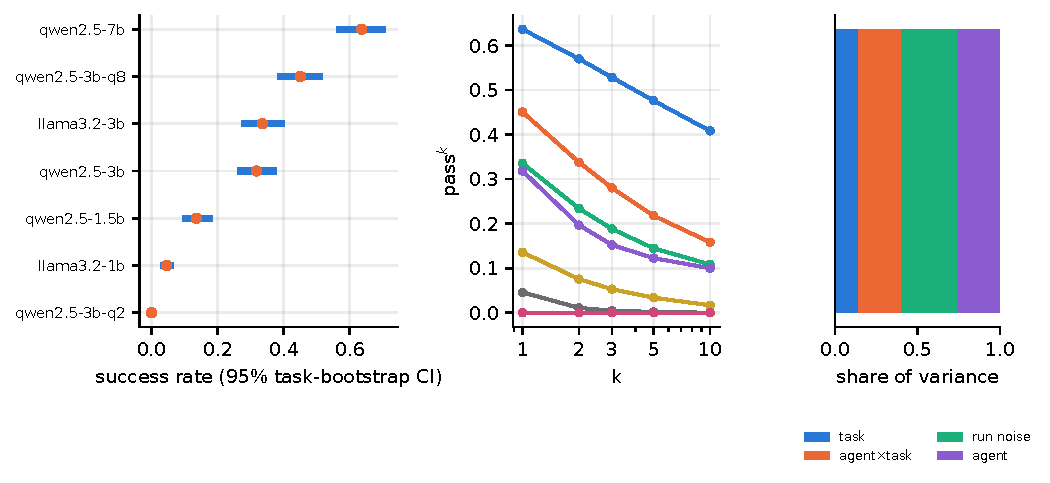
\includegraphics[width=\linewidth]{figures/real_main.pdf}
\caption{Local models on the \realNTasks-task core suite, \realNRuns{} runs per task. Left: success rate with 95\% task-bootstrap interval. Middle: pass$^k$. Right: variance decomposition of the full agents-by-tasks-by-runs array.}\label{fig:real}
\end{figure}

\paragraph{Reliability is much lower than the headline score.} The best model's score of \realBestScore{} falls to \realBestPassThree{} for pass$^3$ and \realBestPassTen{} for pass$^{10}$: a model that solves a task on average does not solve it every time. Run noise accounts for \realRunShare{} of the variance of single runs, task difficulty for \realTaskShare, agent-by-task interaction for \realInterShare{} and agent identity for \realModelShare. The agent share describes the spread of these seven fixed models, not a population variance. Run noise is of the same order as the quantity of interest, so a one-run evaluation is a noisy measurement even here.

\paragraph{Ranking: the hypothesis is only partly borne out.} Because the models differ a lot in capability, the ranking is well determined: \realNIndist{} of \realNPairs{} pairs are not separable after Holm correction (\realClosestA{} versus \realClosestB{}, a gap of \realClosestDiff{} points, adjusted $p=\realClosestP$), and the split-half rank correlation is \realSplitTau. This contrasts with SWE-bench, where scores are close; the statistical problems are most severe when systems are close, not absent otherwise. A plug-in power calculation says that resolving a 5-point difference between two of these agents at 80\% power needs about \realTasksNeeded{} tasks at ten runs per task, more than three times the suite size, and the minimum detectable difference of the current design is \realMDE{} points; both are estimates from one pilot and carry the uncertainty documented for $\tau$-bench above. With the cost model of Section~\ref{sec:power}, the optimal number of runs per task is \realOptRuns{} when a task costs as much as ten runs.

\subsection{Ablations on real data}\label{sec:ablation}
\paragraph{Tasks versus runs.} The sub-designs are random subsets of the same \realNTasks{} tasks and ten runs, compared with the ranking and the significant pairs of the full data. The full-data ranking shares observations with every subsample and is itself an estimate, so this measures \emph{internal stability relative to the full observed sample}, not recovery of an independently known population ranking; the pairs that are significant in the full data are also selected by the same data, so sign agreement among them is optimistic. Recovery of a known ranking is examined in the simulation (E6, Figure~\ref{fig:rankcal}); a split-sample analysis on independent halves would require the per-run outcomes, which are not stored. Sub-sampling the real data (Figure~\ref{fig:realabl}), a ranking from all \realNTasks{} tasks with one run per task has Kendall $\tau=\ablTauOneRun$ with the full-data ranking and separates \ablFracOneRun{} of the pairs, against \ablFracAllRuns{} with ten runs. With only \ablFewTasks{} tasks and one run the ranking correlation is $\tau=\ablTauFewTasks$ and only \ablFracFewTasks{} of pairs are separated. Since the large gaps are easy, rank correlation saturates quickly; the number of \emph{separated pairs} is the informative measure and it keeps growing with both tasks and runs. We did not repeat the fixed-budget comparison of Section~\ref{sec:sim} on real data, so the simulation result on tasks versus runs is neither confirmed nor refuted here.
\begin{figure}[t]
\centering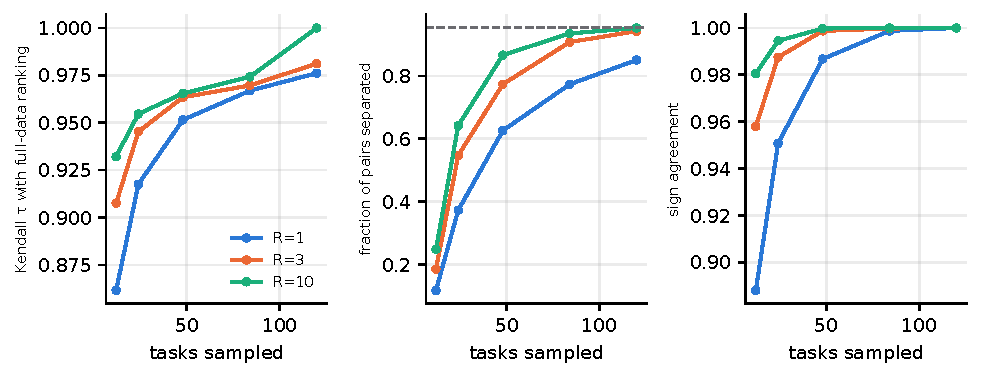
\includegraphics[width=\linewidth]{figures/real_ablation.pdf}
\caption{Sub-designs of the real data (random subsets of tasks and runs, 200 draws). Left: Kendall $\tau$ with the full-data ranking. Middle: fraction of the \realNPairs{} pairs separated (paired $t$-test, Holm); the dashed line is the full data. Right: sign agreement for pairs that are significant in the full data. The reference is the full-data result, which shares observations with every subsample, so all panels measure stability relative to the observed sample, not accuracy against a known truth.}\label{fig:realabl}
\end{figure}

\paragraph{Sequential stopping.} Applying the confidence sequence to tasks in random order, \seqRealDecided{} of the \seqRealNSig{} pairs that are significant on the full data are decided before the tasks run out, with a median of \seqRealMedTasks{} tasks. This re-orders existing results; it is not a live stopping experiment. Large gaps are settled after a few tens of tasks; close pairs are not decided within the suite, as in the simulation.

\paragraph{Cost profile.} Figure~\ref{fig:realprof} reports tokens and wall-clock per run. The weakest functioning model, \realMaxStepLimitModel, hits the step limit in \realMaxStepLimit{} of runs and consumes the most tokens: failure is not cheap, so cost per success varies more than cost per run. Wall-clock was measured with four parallel workers on one machine and is indicative only.
\begin{figure}[t]
\centering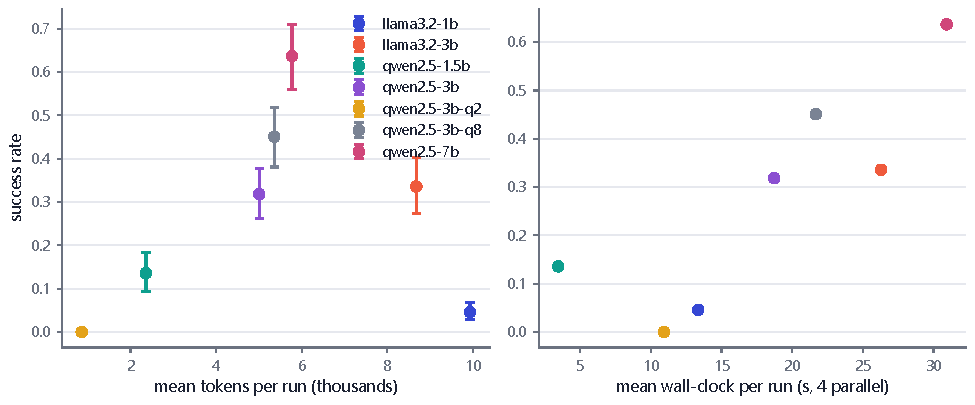
\includegraphics[width=\linewidth]{figures/real_profile.pdf}
\caption{Success rate against mean tokens (left) and wall-clock (right) per run.}\label{fig:realprof}
\end{figure}
